\documentclass{scrartcl}
 
\usepackage[utf8]{inputenc}
\usepackage[T1]{fontenc}
\usepackage{lmodern}
\usepackage[pdftex]{graphicx}
\usepackage[ngerman]{babel}
\usepackage{amsmath}
\usepackage{amssymb}
\usepackage{tabularx}
\usepackage{multirow}
\usepackage{amsfonts}
\usepackage{tabto}
\usepackage{mathtools}
\TabPositions{0.1in, 0.4in, 0.6in, 0.8in, 1.0in, 1.2in, 3.4in}

\begin{document}
\begin{LARGE}
Spieltheorie - WiSe 2014/15
\end{LARGE}

\begin{Large}
Übungsblatt 6 - Felix Dosch\\[1.0cm]
\end{Large}

\begin{Large}
Aufgabe 6.2\\[0.0cm]
\end{Large}

Wir suchen eine konvergente Folge von Strategievektoren
$\sigma^k$, sodass jeder dieser Strategievektoren im $\epsilon^k$-pertubierten Spiel $\Gamma^k$ ein
Nash-Gleichgewicht ist. \\

Zunächst brauchen wir eine Folge von $\epsilon_i$-Pertubationsvektoren, welche die Voraussetzungen der
Definition des perfekten Nash-Gleichgewichts aus der Vorlesung erfüllen:
\[
\lim_{k \to \infty} M(\epsilon^k) = 0 \quad \text{mit } M(\epsilon) = \max_{i \in N,s_i \in S_i}
{\epsilon_i(s_i)}
\]

Der Einfachheit halber definieren wir die Folge $\epsilon^k_{i} = \frac{1}{k+|S_i|}$ für alle 
$k \in \mathbb{N}$ und für alle $i \in S_i$. Diese konvergiert offensichtlich für jeden Spieler nach 0,
womit $\lim_{k \to \infty} M(\epsilon^k) = 0$ erfüllt ist für $\epsilon =$ Vektor der
Pertubationsvektoren für alle Spieler.$^1$

Da $B$ eine schwach dominierte Strategie ist, wird Spieler I immer so viel $T$ wie möglich spielen
und nur gerade so viel $B$ wie unbedingt nötig ($\sigma^k_I(B) = \epsilon^k_I(B)$)$^2$. Für Strategie
$T$ hat er einen Gewinn von 1 garantiert, für $B$ kommt es auf die Strategie von II an. Daher gibt 
es keinen Grund, für I mehr $B$ zu spielen, unabhängig von Spieler II.

Für Spieler II macht es daher nun Sinn, Strategie $L$ zu spielen, so viel er kann, und $M$ nur gerade
so viel wie nötig ($\sigma^k_{II}(M) = \epsilon^k_{II}(M)$)$^3$ und davon nicht abzuweichen. Daher ist
(T, L) im Ausgangsspiel ein Nash-Equilibrium$^4$, und sogar das einzige Nash-Equilibrium (Angenommen
Spieler I spielt nicht $T$, dann macht es immer Sinn, zu $T$ zu wechseln, da dort der erwartete Gewinn 
höher ist - Angenommen I spielt $T$ und II spielt nicht $L$, dann ist der erwartete Gewinn für II in $L$ 
höher, also sollte er zu $L$ wechseln).$^5$\\

Wir behaupten also, dass $\sigma = (T, L)$ das einzige perfekte Nash-Gleichgewicht ist. \\

$\xRightarrow{2,3}$ Für das Spiel $\Gamma^k$ ist ($\sigma^k_I = ((1 - \epsilon^k_I) \cdot T, \epsilon^k_I 
\cdot B), \sigma^k_{II} = ((1 - \epsilon^k_{II}) \cdot L, \epsilon^k_{II} \cdot M))$ ein 
Nash-Equilibrum.$^6$
\\

$\xRightarrow{4,6} \lim_{k \to \infty} \sigma^k = ((1 \cdot T, 0 \cdot B), (1 \cdot L, 0 \cdot M)) =
\sigma$ ist ein Nash-Equilibrium.$^7$ \\

$\xRightarrow{1,5,7} \sigma = (T, L)$ ist ein perfektes Nash-Gleichgewicht und sogar das einzige (da ein
perfektes Nash-Gleichgewicht immer ein Nash-Gleichgewicht ist (s. Vorlesung). \clearpage

\begin{Large}
Aufgabe 6.3\\[0.0cm]
\end{Large}

a) Für das strikte symmetrische Nash-Gleichgewicht $(\sigma', \sigma')$ gilt: 

\[
\forall i \in \{I, II\} \quad \forall \sigma_i \in \Sigma_i \setminus \{\sigma'\} : u_i(\sigma_i, 
\sigma') < u_i(\sigma', \sigma') 
\]

Dies erfüllt genau eine der äquivalenten Definitionen für die ESS aus der Vorlesung: \\

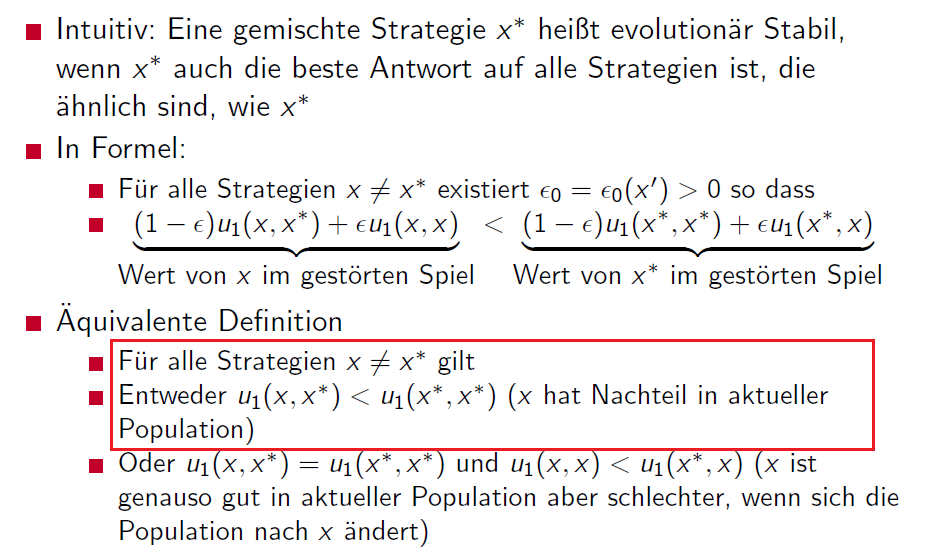
\includegraphics[width=14.5cm]{ess_def.png} \\

b) Beweis durch Widerspruch: Angenommen $\sigma^* \neq \sigma'$. \\

$\sigma^*$ ESS $\Rightarrow \sigma^*$ Nash-GG $\Rightarrow u_1(\sigma^*, \sigma^*) \geq u_1(\sigma',
\sigma^*)$. \\

Da $\sigma'$ beste Antwort auf $\sigma^* \Rightarrow u_1(\sigma^*, \sigma^*) = u_1(\sigma',
\sigma^*)$. \\

Da $\sigma^*$ ESS muss gelten $u_1(\sigma',\sigma') < u_1(\sigma', \sigma^*)$ (siehe äquivalente Def.
für ESS aus Vorlesung). \\

Widerspruch, da $(\sigma',\sigma')$ Nash-Gleichgewicht. Daher ist die Annahme falsch und es gilt
$\sigma^* = \sigma'$. \\

\end{document}